\documentclass[a4paper,12pt]{book}

\usepackage{ZeroSeven}

\titlepage{}

\author{Mirko Franco}
\date{26-11-2018}
\intestazioni{
\includegraphics[scale=0.3]{images/logo_intestazione}}
\pagestyle{myfront}
\begin{document}
\begin{titlepage}
	\centering
	{\huge\bfseries MegAlexa\par}
	Arricchitore di skill di Amazon Alexa
	\line(1,0){350} \\
	{\scshape\LARGE Nome documento \par}
	\vspace{1cm}
	{\scshape Gruppo ZeroSeven \par}
	\logo
	%devono essere compilati questi campi ogni volta
	\begin{tabular}{c|c}
		{\hfill \textbf{Versione}} 			& 0.0.1				\\
		{\hfill\textbf{Data Redazione}} 	& 24-12-2018		\\ 
		{\hfill\textbf{Redazione}} 			&  		Stefano Zanatta			\\ 
		{\hfill\textbf{Verifica}} 				&  	Andrea Deidda			\\ 
		{\hfill\textbf{Approvazione}} 		&  		Stefano Zanatta			\\ 
		{\hfill\textbf{Uso}} 					& 		Esterno		\\ 
		{\hfill\textbf{Distribuzione}} 			& 			Prof. Tullio Vardanega \\ & Prof. Riccardo Cardin \\ & Gruppo ZeroSeven		\\ 
		{\hfill\textbf{Email di contatto}} & zerosevenswe@gmail.com \\
	\end{tabular}
\end{titlepage}
	

	
	\label{LastFrontPage}
	\newpage	
	\begin{center}
	\textbf{Registro delle modifiche}
	\end{center}
	\begin{center}
		\begin{tabularx}{\textwidth}{|c|c|X|X|c|}
			\hline
			\textbf{Versione} & \textbf{Data} & \textbf{Descrizione} & \textbf{Autore} & \textbf{Ruolo} \\ 
			\hline
			3.0.0 & 2019-04-11 & Approvazione per il rilascio RQ & Ludovico Brocca & Responsabile \\
			\hline
			2.1.0 & 2019-04-09 & Verifica documento & Ludovico Brocca & Verificatore \\
			\hline
			2.0.6 & 2019-04-08 & Aggiunto riferimento metriche alla sezione \S\ref{MetricheObbiettivi} &Matteo depascale & Amministratore \\
			\hline 
			2.0.5 & 2019-04-08 & Modifica sezioni \S\ref{Verifica}  e \S\ref{Validazione} & Matteo depascale & Amministratore \\
			\hline
			2.0.4 & 2019-04-08 & Aggiunti comandi personalizzati alla sezione \S\ref{NormeRedazionali} &Matteo depascale & Amministratore \\
			\hline
			2.0.3 & 2019-04-04 & Aggiunta voci a \S\ref{ListaControllo} & Matteo depascale & Amministratore \\
			\hline
			2.0.2 & 2019-04-01 & Stesura sezioni \S\ref{DiagrammiDelleClassi}, \S\ref{DiagrammiPackage}, \S\ref{DiagrammiSequenza} e \S\ref{DiagrammiAttivita}  & Bianca Andreea Ciuche & Amministratore \\
			\hline
			2.0.1 & 2019-03-23 & Modifica \ref{Documentazione fornita} Corretti numeri di sezione & Bianca Andreea Ciuche & Amministratore \\
			\hline
			2.0.0 &2019-03-07 & Approvazione per il rilascio & Gian Marco Bratzu& Responsabile\\
			\hline
			1.2.0 &2019-03-02 & Verifica documento &Andrea Deidda& Verificatore\\
			\hline
			1.1.2 &2019-02-13 &Stesura \S\ref{calcoloOre} &Ludovico Brocca& Amministratore\\
			\hline
			1.1.1 &2019-02-13 &Modifica\S \ref{anDinamica} &Ludovico Brocca& Amministratore\\
			\hline
			1.1.0 &2019-02-07 &Verifica \S\ref{processo}, \ref{metriche}, \S\ref{progettazione} &Gian Marco Bratzu& Verificatore\\
			\hline
			1.0.4 &2019-02-04&Stesura \S\ref{processo}&Ludovico Brocca& Analista\\
			\hline
			1.0.3 & 2019-02-03 & Modifica \S\ref{metriche} & Stefano Zanatta & Amministratore\\
			\hline
			1.0.2 & 2019-02-02 & Stesura \S\ref{metriche} & Bianca Andreea Ciuche & Amministratore\\
			\hline
			1.0.1 & 2018-01-12 & Stesura \S\ref{progettazione} & Mirko Franco & Amministratore \\
			\hline
			1.0.0 & 2018-01-09 & Approvazione per il rilascio & Stefano Zanatta & Responsabile\\
			\hline
			0.2.0 & 2018-12-29 & Verifica documento & Stefano Zanatta & Verificatore\\
			\hline
			0.1.0 & 2018-12-18 & Verifica \S\ref{PdS} & Mirko Franco & Verificatore\\
			\hline
			0.0.6 & 2018-12-21 & Modifica \S\ref{Intro} & Andrea Deidda & Amministratore\\
			\hline
			0.0.5 & 2018-12-17 & Stesura \S\ref{Po} & Ludovico Brocca & Amministratore\\
			\hline
			0.0.4 & 2018-12-16 & Stesura \S\ref{Pp} & Matteo Depascale & Amministratore\\
			\hline
			0.0.3 & 2018-12-16 & Stesura \S\ref{Intro} & Bianca Ciuche & Amministratore\\
			\hline
			0.0.2 & 2018-12-10 & Stesura \S\ref{PdS} & Gian Marco Bratzu & Amministratore\\	
			\hline
			0.0.1 & 2018-12-08 & Struttura documento  & Ludovico Brocca & Amministratore\\
			\hline
	\end{tabularx}
	\end{center}

\newpage
	\pagestyle{mymain}
	\tableofcontents
	\chapter{Introduzione}
\label{introduzione}
\section{Scopo del documento}
Il \textit{Piano di Qualifica} ha lo scopo di definire gli obbiettivi di qualità che il gruppo perseguita per il proprio prodotto. Per ottenere tali obbiettivi è necessario un processo di verifica continua di ogni attività. Questo consente di rilevare e correggere le anomalie riscontrate tempestivamente.\\
Questo documento descrive nel dettaglio la qualità dei processi più vicini nel tempo e ad alto livello quelli più lontani, per poi essere aggiornato con nuovi contenuti ogni volta che il gruppo lo ritiene necessario.
\section{Scopo del prodotto}
Lo scopo del progetto è quello di sviluppare un applicativo Mobile in grado di creare delle routine personalizzate per gli utenti gestibili tramite\glossario{Alexa}di\glossario{Amazon}. L'obbiettivo è quello di creare\glossario{skill}in grado di avviare\glossario{workflow}creati dagli utenti fornendogli dei\glossario{connettori}.
\section{Glossario}
Al fine di evitare ogni ambiguità di linguaggio e massimizzare la comprensione dei documenti, i termini tecnici, di dominio, gli acronimi e le parole che necessitano di essere chiarite, sono riportate nel \textit{Glossario v1.0.0}.\\
Ogni occorrenza di vocaboli presenti nel \textit{Glossario} è marcata da una "G" maiuscola in pedice.
\section{Riferimenti}
\subsection{Normativi}
\begin{itemize}
	\item  \textbf{Norme di Progetto}: \textit{Norme di Progetto v1.0.0};
	\item \textbf{Capitolato$_{G}$ C4}:\glossario{MegAlexa}: arricchitore di skill di Amazon Alexa.
	\item \textbf{Ciclo di Deming}
	\footnote{\url{https://it.wikipedia.org/wiki/Ciclo_di_Deming}}
\end{itemize}
\subsection{Informativi}\label{rfinf}
\begin{itemize}
	\item \textbf{Piano di Progetto}: \textit{Piano di Progetto v1.0.0};
	\item \textbf{Complessità ciclomatica}
	\item \textbf{Software Testing Fundamentals: Methods and Metrics} di Marnie L. Hutcheson, Wiley Publishing, Inc.  
	\footnote{\url{https://www.math.unipd.it/~tullio/IS-1/2018/Progetto/C4.pdf}}.
	
	
\end{itemize}

	\chapter{Qualità di Processo}
\section{Obbiettivi}
Affinché la qualità di prodotto sia garantita è necessario perseguire al qualità dei processi che concorrono alla sua realizzazione. Per raggiungere questo obbiettivo viene adottato lo standard ISO/IEC 15504 denominato SPICE che fornisce strumenti per valutare la bontà dei processi che vengono realizzati.
Per applicare correttamente questo standard è necessario utilizzare il ciclo di Deming (ciclo PCDA) che fornisce una metodologia per il controllo dei processi che consente di migliorarne in modo continuativo la qualità. 
\section{Procedure di controllo di qualità dei processi}
La qualità dei processi viene garantita dall'applicazione del ciclo PDCA. Grazie a tale principio è possibile ottenere un miglioramento continuo della qualità di ogni processo e come diretta conseguenza si ottiene il miglioramento dei prodotti ottenuti.
Per avere controllo dei processi, e di conseguenza migliorarne la qualità, bisogna: 
\begin{itemize}
		\item Definire in modo dettagliato i processi;
		\item Assegnare in modo chiaro le risorse ai processi;
		\item Avere controllo sui processi.
\end{itemize} 
La realizzazione di questi punti è descritta in modo dettagliato nel \textit{Piano di Progetto v1.0.0}.
\section{Metriche}
Come metrica per i processi si è deciso di utilizzare indici che ci permettano di valutare costi e tempi. 
\subsection{Schedule Variance (SV)}
Indica se si è in linea, in anticipo o in ritardo rispetto alla pianificazione temporale indicata delle attività. 
Se SV > 0 significa che il gruppo sta procedendo con maggiore velocità rispetto a quanto pianificato, viceversa se negativo. 
Essendo stati inseriti slack durante la pianificazione delle attività dei processi, il valore di tale indice è inizialmente positivo.
\subsection{Budget Variance (BV)}
	\chapter{Qualità di Prodotto}

\section{Qualità dei documenti}
I documenti prodotti dal gruppo ZeroSeven devono essere leggibili e corretti. Vengono utilizzate le seguenti metriche, definite nelle \textit{Norme di Progetto}:
\begin{itemize}
    \item \textbf{MD001 Indice di Gulpease};
    \item \textbf{MD002 Ortografia};
    \item \textbf{MD003 Formula di Flesch:} per i Dialog Flow descritti nell' \textit{Analisi dei Requisiti}.
\end{itemize}

\section{Qualità del software}
Segue una descrizione dettagliata delle metriche stabilite dal gruppo per perseguire obbiettivi di qualità software. \newline
Esse costituiscono una dichiarazione d'intenti, e potrà subire modifiche nelle revisioni successive.
\subsection{Complessità ciclomatica}
Metrica software che indica la complessità di un programma tenedo in considerazione \glossario{moduli}, \glossario{funzioni}, \glossario{metodi} e \glossario{classi}.
Nello specifico, essa è calcolata tramite il grafo di controllo di flusso del programma, dove i nodi sono gruppi indivisibili di istruzioni e gli archi connettono due nodi se il secondo gruppo di istruzioni può essere eseguito immediatamente dopo il primo , e il suo valore è determinato dal numero di cammini linearmente indipendenti all'interno del codice sorgente. 
\'E quindi opportuno definire un valore di complessità ciclomatica preciso: valori alti sono indice di scarsa manutenibilità del codice e valori bassi potrebbero indicare scarsa efficienza dei metodi.
Esso fornisce, inoltre, un indice del carico di lavoro richiesto per la fase di testing (un valore alto richiede più test per una copertura completa).
Il range di ottimalità stabilito varia da 0 a 10, come suggerito dall'ideatore della materica Thomas J. McCabe.  





\section{Tabella delle metriche}
\begin{center}
	\begin{tabularx}{\textwidth}{|c|X|c|c|}
		\hline
		\textbf{Codice} & \textbf{Nome} & \textbf{Range di accettazione} & \textbf{Range di ottimalità} \\
		\hline
		MD001 & Indice di Gulpease & 50-100 &60-100\\
		MD002 &Ortografia & 100-100 & 100-100\\
		MD003 &Formula di Flesch& 75-100 &80-100 \\
		\hline
		MS001 & Complessità ciclomatica & 0-16 & 0-10 \\
		
		
	\end{tabularx}
\end{center}
	\input{sezioni/qualita_test}
	\chapter{Resoconto delle attività di verifica}
\label{resoconto}
\section{Analisi}
Nel periodo antecedente la Revisione dei Requisiti sono stati verificati i documenti ed i processi applicando quanto descritto nelle \textit{Norme di Progetto v2.0.0}.\\
L'analisi statica è stata effettuata secondo i criteri e le modalità indicate nelle \textit{Norme di Progetto}.\\ 
Per gli errori riscontrati effettuando \textit{walkthrough$_{G}$}, si è provveduto a correggere le anomalie riscontrate e sono stati riportati nella lista di controllo nelle \textit{Norme di Progetto v2.0.0} per permettere di effettuare inspection successivamente.\\
L'\textit{inspection$_{G}$} viene effettuata utilizzando la lista di controllo precedentemente stilata. \\
Si sono poi calcolate le metriche descritte nelle \textit{Norme di Progetto}.\\
L'avanzamento dei processi viene poi valutato secondo le metriche descritte nelle \textit{Norme di Progetto}. 
\subsection{Verifica dei processi}
Per il\glossario{processo}di stesura dei documenti, il calcolo delle metriche di Budget Variance e di Schedule Variance è stato effettuato sul valore complessivo delle ore impiegate dal totale dei componenti del gruppo.\\
Per le successive fasi del \textit{progetto$_{G}$}, il gruppo si propone di automatizzare il processo di calcolo delle ore impiegate, con il dettaglio puntuale dei singoli processi.
Lo Schedule Variance totale è di -1 ore e il Budget Variance totale equivale a -25\euro.
\begin{comment}
\begin{tabularx}{\textwidth}{|C|C|C|}
	\hline
	\textbf{Macro-Attività}& \textbf{SV}&\textbf{BV}\\
	\hline
	\textit{Norme di Progetto}    & \euro & \euro\\
	\textit{Piano di Progetto}    & \euro & \euro\\
	\textit{Studio di Fattibilità} & \euro & \euro\\
	\textit{Analisi dei Requisiti}& \euro & \euro\\
	\textit{Piano di Qualifica}   & \euro & \euro\\
	\textit{Glossario}            & \euro & \euro\\
	\hline
	\caption{Esito verifica processi}
\end{tabularx}
\end{comment}
\\
\subsection{Verifica dei documenti}
\begin{tabularx}{\textwidth}{|C|c|C|}
	\hline
	\textbf{Documento}& \textbf{Indice di Gulpease}&\textbf{Esito}\\
	\hline
	\endhead
	\textit{Norme di Progetto}    & 76 & Superato \\
	\textit{Piano di Progetto}    & 64 & Superato \\
	\textit{Studio di Fattibilità} & 61 & Superato\\
	\textit{Analisi dei Requisiti}& 80 & Superato \\
	\textit{Piano di Qualifica}   & 67 & Superato \\
	\textit{Glossario}            & 68 & Superato \\
	\hline
	\caption{Esito della verifica documenti}
\end{tabularx}

\section{Revisione Analisi}
\label{revisione}
Durante il breve periodo di Revisione Analisi, il gruppo si è preparato allo sviluppo del POC e ha apportato delle correzione ai documenti, migliorando i propri processi. 
\subsection{Verifica dei processi}
I miglioramenti principali (tutti descritti nelle \textit{Norme di Progetto v2.0.0}) sono stati:
\begin{itemize}
	\item Automatizzato il calcolo delle ore di lavoro integrando \glossario{Harvest} ad \glossario{Asana};
	\item Automatizzato il calcolo dell'indice di Gulpease, tramite script;
	\item Se dei documenti contenenti degli errori grammaticali raggiungono la repository, un bot avvisa per email chi ha commesso l'errore e invia una notifica al gruppo.
\end{itemize}

\subsubsection{MP001 Schedule variance}
\begin{figure} [h]
    \centering
	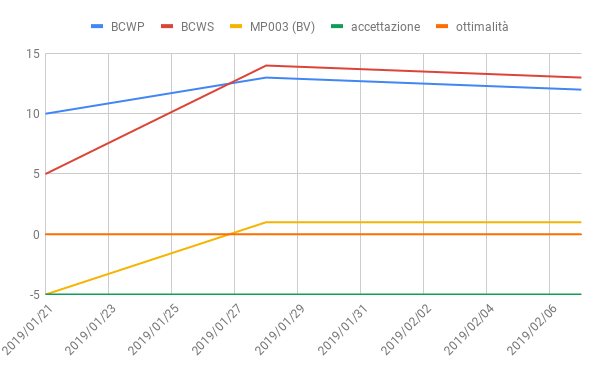
\includegraphics[scale=0.5]{./images/svRa.png}
	\caption{\textit{MP001 - Revisione Analisi}}\label{}
\end{figure}
\pagebreak
\subsubsection{MP002 Budget variance}
\begin{figure} [h]
    \centering
	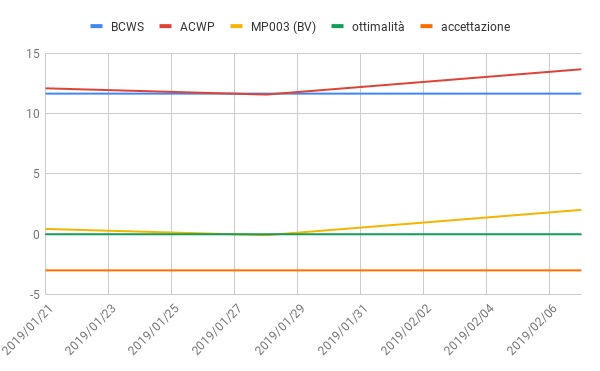
\includegraphics[scale=0.5]{./images/bvra.png}
	\caption{\textit{MP002 - Revisione Analisi}}\label{}
\end{figure}

\section{Progettazione della base tecnologica}
\label{progettazione}
\subsection{MP001: Schedule variance}
\begin{figure} [h]
    \centering
	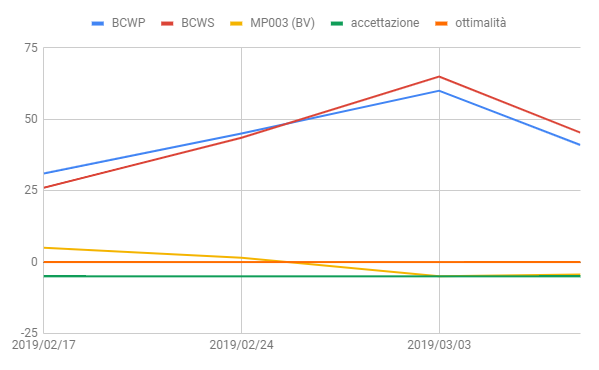
\includegraphics[scale=0.5]{./images/svP.png}
	\caption{\textit{MP001 - Progettazione della base tecnologica}}\label{}
\end{figure}
\pagebreak
\subsection{MP002: Budget variance}
\begin{figure} [h]
    \centering
	\includegraphics[scale=0.5]{./images/bvP.png}
	\caption{\textit{MP002 - Progettazione della base tecnologica}}\label{}
\end{figure}

\subsection{MP003: SPICE capability level}
Di seguito vengono riportati i livelli di maturità raggiunti dai processi eseguiti durante lo sviluppo del \glossario{poc}. Data l'inesperienza, non viene raggiunto il livello di accettazione richiesto (3) per la maggior parte dei processi, ma il gruppo sta lavorando per migliorare.
\begin{figure} [h]
    \centering
	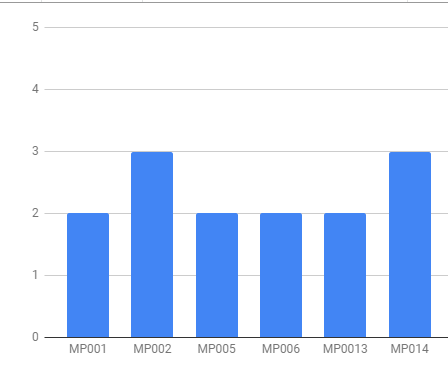
\includegraphics[scale=0.5]{./images/15504.png}
    \caption{\textit{MP003 - ISO/IEC 15504 }}\label{}
\end{figure}

\subsection{MP005:  Occorrenza rischi non previsti}
\textbf{rischi non previsti: 2}
\begin{itemize}
	\item Un aggiornamento automatico di \glossario{Android Studio} ha completamente rimosso una libreria utilizzata dall'applicazione mobile, quindi il gruppo ha perso tempo per implementane una alternativa. Questo è successo perché la libreria in questione era deprecata. Per evitare problemi simili, l'utilizzo di librerie deprecate è stato vietato, come descritto nelle \textit{Norme di Progetto};
	\item E' stata inserita una chiave di accesso Amazon nel repository. Il gruppo è stato avvisato da Amazon, e ha dovuto creare nuove chiavi per tutti i membri.
\end{itemize}

\subsection{MP006: Indisponibilità dei servizi}
\textbf{indisponibilità dei servizi: 0}\\
Durante il periodo di progettazione della base tecnologica, il gruppo non ha riscontrato problemi riguardanti il downtime di servizi esterni.

\subsection{MP013: Percentuale build superate}
Viene fatta distinzione tra Android e Skill, in quanto vengono contenute in repository diversi.\\
Le build non superate sono 24 su 134 per la Skill e 29 su 232 per Android. Entrambe superano il range di ottimalità (80\%);
\begin{figure} [h]
    \centering
	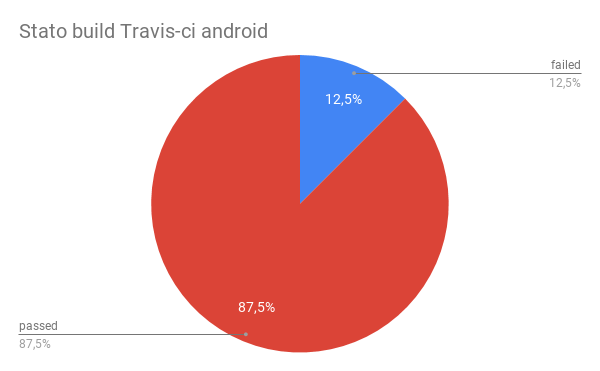
\includegraphics[scale=0.5]{./images/StatobuildTravis-ciandroid.png}
    \caption{\textit{MP013 - Android - Progettazione della base tecnologica}}\label{}
\end{figure}\\
\begin{figure} [h]
    \centering
	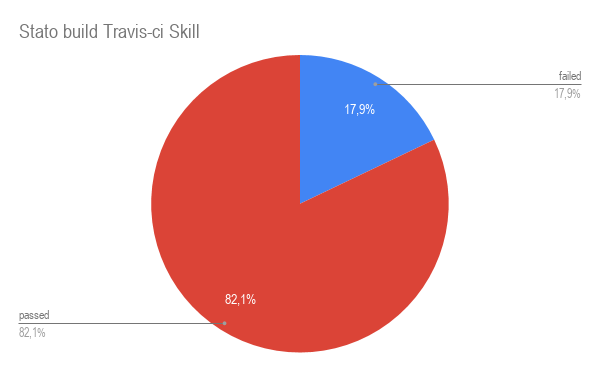
\includegraphics[scale=0.5]{./images/StatobuildTravis-ciSkill.png}
    \caption{\textit{MP013 - Skill - Progettazione della base tecnologica}}\label{}
\end{figure}
\clearpage

\subsection{MP014: Media commit giornaliera}
Come si può vedere dai grafici, il numero di commit è stato abbastanza costante, con un aumento del carico di lavoro durante la fine di febbraio.
\begin{figure} [h]
    \centering
	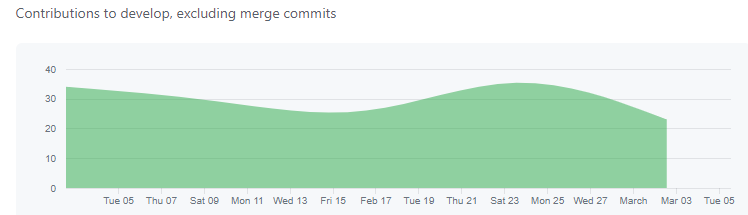
\includegraphics[scale=0.5]{./images/dailycommits_kotlin.PNG}
    \caption{\textit{MP014 - Android- Progettazione della base tecnologica}}\label{}
\end{figure}
\begin{figure} [h]
    \centering
	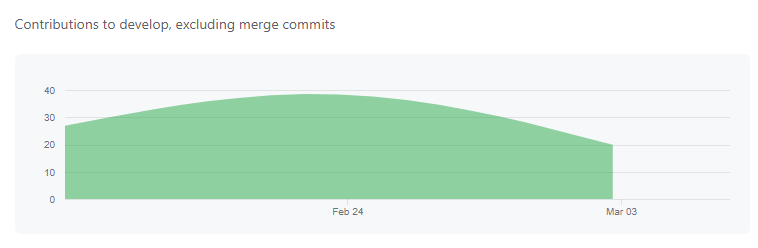
\includegraphics[scale=0.5]{./images/daycommits_js.PNG}
    \caption{\textit{MP014 - Skill - Progettazione della base tecnologica}}\label{}
\end{figure}

\subsection{MP015, MP016: Percentuale requisiti soddisfatti}
\begin{figure} [h]
    \centering
	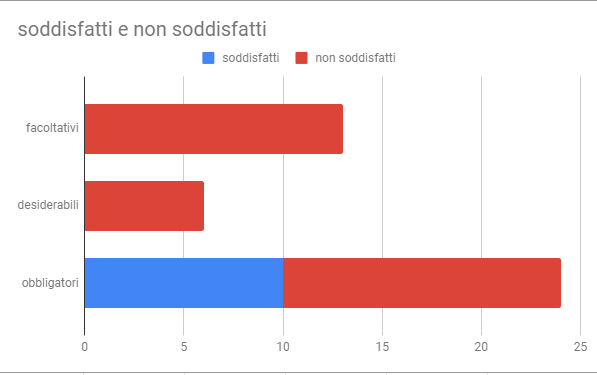
\includegraphics[scale=0.5]{./images/req.PNG}
    \caption{\textit{MP015 - MP016 Tipologia di requisiti}}\label{}
\end{figure}
\begin{figure} [h]
    \centering
	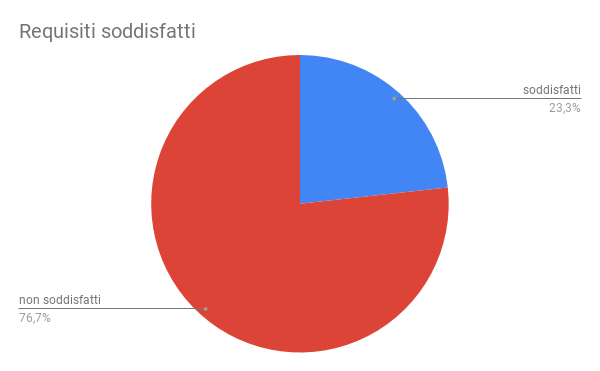
\includegraphics[scale=0.5]{./images/RequisitiSoddisfatti.png}
    \caption{\textit{MP015 - MP015 Differenza soddisfatti e non soddisfatti}}\label{}
\end{figure}

\newpage
\section{Progettazione di dettaglio e codifica}
Questa sezione verrà compilata alla fine del periodo di Progettazione della base tecnologica.
\section{Verifica e collaudo}
Questa sezione verrà compilata alla fine del periodo di Verifica e collaudo.

			
	\label{LastPage}

\end{document}